\section{Vergleich von AdaBoost und Gradient Boosting}
In diesem Abschnitt werden die Unterschiede zwischen den Boosting-Algorithmen AdaBoost und Gradient Boosting (GBT) diskutiert. Wir betrachten ihre theoretischen Grundlagen, praktische Umsetzung, Vor- und Nachteile sowie typische Anwendungsfälle.

\subsection{Theoretische Grundlagen}
AdaBoost und GBT sind beides Ensemble-Lernmethoden, die auf dem Prinzip des Boosting basieren. AdaBoost konzentriert sich darauf, die Gewichte von Trainingsdaten anzupassen, um die Fehler der vorherigen Lerner zu korrigieren. Dies führt zu einer sequenziellen Anpassung, bei der jeder nachfolgende Lerner versucht, die Schwächen des Vorgängers zu verbessern. 
\newline
\newline
Im Gegensatz dazu arbeitet GBT mit Entscheidungsbäumen und konzentriert sich auf die Minimierung einer differenzierbaren Verlustfunktion, häufig unter Verwendung von Gradientenabstiegsverfahren. Dieser Ansatz ermöglicht es GBT, sowohl für Klassifikations- als auch für Regressionsprobleme effektiv zu sein.

\subsection{Praktische Umsetzung}
In der praktischen Anwendung wird AdaBoost häufig bei binären Klassifikationsproblemen eingesetzt, während GBT seine Stärken in komplexen Regressionsproblemen und multiklassen Klassifikationsaufgaben zeigt. AdaBoost ist in der Regel schneller in der Trainingsphase, da es einfacher in seiner Struktur ist. GBT hingegen, kann durch seine Flexibilität in der Anpassung von Entscheidungsbäumen und Verlustfunktionen komplexere Muster in den Daten erfassen.

\subsection{Vor- und Nachteile}
Ein wesentlicher Vorteil von AdaBoost liegt in seiner Einfachheit und Effizienz. Es ist leicht zu implementieren und bietet gute Ergebnisse bei einer Vielzahl von Problemen. Allerdings ist AdaBoost anfällig für Überanpassung, insbesondere bei Rauschen und Ausreißern in den Daten.
\newline
\newline
GBT hingegen ist flexibler und leistungsfähiger bei der Handhabung verschiedener Arten von Datenstrukturen und Verteilungen. Es kann jedoch rechenintensiver sein und erfordert eine sorgfältigere Abstimmung der Hyperparameter.

\subsection{Einsatzgebiete und Leistungsbewertung}
AdaBoost wird häufig in Anwendungen eingesetzt, bei denen die Geschwindigkeit der Modellerstellung kritisch ist und die Daten relativ frei von Ausreißern sind. GBT hingegen findet Anwendung in Szenarien, bei denen die Genauigkeit des Modells von höchster Bedeutung ist, wie beispielsweise in fortgeschrittenen Analytiken oder bei komplexen Regressionsproblemen.

\subsubsection{Datensatz `california housing'}
Um diese Unterschiede zu veranschaulichen habe ich mich für eine komplexe Regressiononsaufgabe, den bekannten Datensatz zu den Wohnungsdaten in Kalifornien, entschieden. Ziel bei diesem Datensatz ist es, den Hauspreis zu schätzen.

\begin{table}[ht]
    \centering
    \caption{Beispieldaten aus dem Kalifornien Wohnungsdatensatz}
    \label{tab:housing_data}
    \resizebox{\textwidth}{!}{
    \begin{tabular}{rrrrrrrrr}
\toprule
MedInc & HouseAge & AveRooms & AveBedrms & Population & AveOccup & Latitude & Longitude & Hauspreis \\
\midrule
8.33 & 41.00 & 6.98 & 1.02 & 322.00 & 2.56 & 37.88 & -122.23 & 4.53 \\
8.30 & 21.00 & 6.24 & 0.97 & 2401.00 & 2.11 & 37.86 & -122.22 & 3.58 \\
7.26 & 52.00 & 8.29 & 1.07 & 496.00 & 2.80 & 37.85 & -122.24 & 3.52 \\
5.64 & 52.00 & 5.82 & 1.07 & 558.00 & 2.55 & 37.85 & -122.25 & 3.41 \\
3.85 & 52.00 & 6.28 & 1.08 & 565.00 & 2.18 & 37.85 & -122.25 & 3.42 \\
\bottomrule
\end{tabular}

    }
\end{table}
    

\begin{figure}[ht]
    \centering
    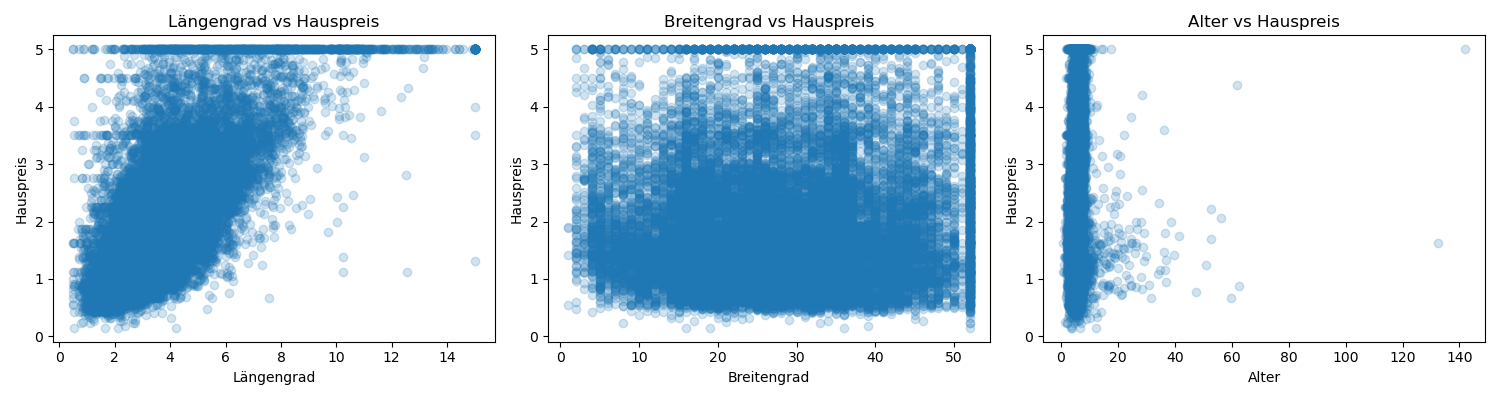
\includegraphics[width=\textwidth]{Images/housing_features.png}
    \caption{Visualisierung von Merkmalen des Kalifornien Wohnungsdatensatzes}
    \label{fig:housing_features}
\end{figure}

\subsubsection{Leistungsvergleich}
Abbildung \ref{fig:housing_performance} zeigt einen Vergleich der Leistung von AdaBoost und GBT auf `california housing' Datensatz. Es wird deutlich, dass GBT in Bezug auf den mittleren quadratischen Fehler (MSE) besser abschneidet, was seine Eignung für komplexe Regressionsprobleme unterstreicht. Allerdings ist AdaBoost deutlich schneller bei der Berechnung gewesen. Auf einem für AdaBoost besser geeigneten Datensatz wäre also GBT weniger effizient.

\begin{figure}[ht]
    \centering
    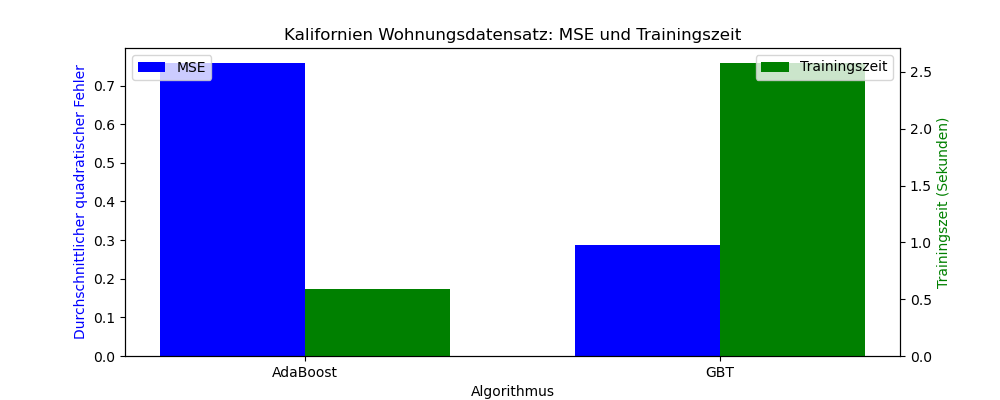
\includegraphics[width=0.8\textwidth]{Images/housing_performance.png}
    \caption{Leistungsvergleich von AdaBoost und GBT auf dem Kalifornien Wohnungsdatensatz}
    \label{fig:housing_performance}
\end{figure}
